\documentclass{minimal}

\usepackage{amsmath}
\usepackage{calc}
\usepackage{tikz}
\usetikzlibrary{arrows,shapes,decorations,positioning,
				decorations.pathmorphing,decorations.pathreplacing,
				automata,backgrounds,
				petri,topaths,trees,
				fit,circuits.ee.IEC}	%To use diverse features from tikz		

\begin{document}
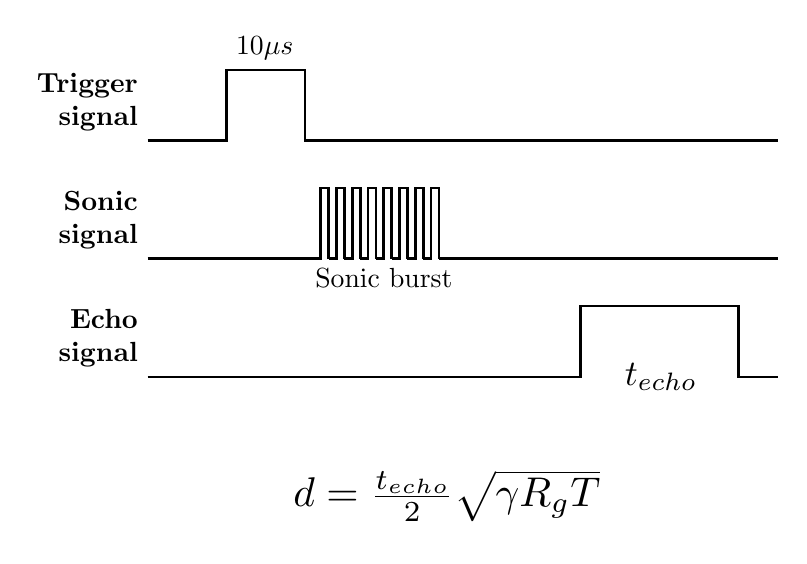
\begin{tikzpicture}

	\node[anchor=east,align=right](trigger){\bfseries Trigger\\ \bfseries signal};
		\coordinate (coordtrig1) at ($(trigger.south east)+(1cm,0)$);
		\coordinate (coordtrig2) at ($(trigger.south east)+(1cm,0.9cm)$);
		\coordinate (coordtrig3) at ($(trigger.south east)+(2cm,0.9cm)$);
		\coordinate (coordtrig4) at ($(trigger.south east)+(2cm,0)$);
		\coordinate (coordtrig5) at ($(trigger.south east)+(8cm,0)$);
		\node[anchor=south west] at (coordtrig2) {10$\mu s$};

	\node[below=1.5cm of trigger.east,anchor=east,align=right](sonic){\bfseries Sonic\\ \bfseries signal};
		\coordinate (coordsonic1) at ($(sonic.south east)+(2.2cm,0)$);
		\coordinate (coordsonic2) at ($(sonic.south east)+(2.2cm,0.9cm)$);
		\coordinate (coordsonic3) at ($(sonic.south east)+(2.3cm,0.9cm)$);
		\coordinate (coordsonic4) at ($(sonic.south east)+(2.3cm,0)$);
		\coordinate (coordsonic5) at ($(sonic.south east)+(2.4cm,0)$);
		\coordinate (coordsonic6) at ($(sonic.south east)+(2.4cm,0.9cm)$);
		\coordinate (coordsonic7) at ($(sonic.south east)+(2.5cm,0.9cm)$);
		\coordinate (coordsonic8) at ($(sonic.south east)+(2.5cm,0)$);
		\coordinate (coordsonic9) at ($(sonic.south east)+(2.6cm,0)$);
		\coordinate (coordsonic10) at ($(sonic.south east)+(2.6cm,0.9cm)$);
		\coordinate (coordsonic11) at ($(sonic.south east)+(2.7cm,0.9cm)$);
		\coordinate (coordsonic12) at ($(sonic.south east)+(2.7cm,0)$);
		\coordinate (coordsonic13) at ($(sonic.south east)+(2.8cm,0)$);
		\coordinate (coordsonic14) at ($(sonic.south east)+(2.8cm,0.9cm)$);
		\coordinate (coordsonic15) at ($(sonic.south east)+(2.9cm,0.9cm)$);
		\coordinate (coordsonic16) at ($(sonic.south east)+(2.9cm,0)$);
		\coordinate (coordsonic17) at ($(sonic.south east)+(3.0cm,0)$);
		\coordinate (coordsonic18) at ($(sonic.south east)+(3.0cm,0.9cm)$);
		\coordinate (coordsonic19) at ($(sonic.south east)+(3.1cm,0.9cm)$);
		\coordinate (coordsonic20) at ($(sonic.south east)+(3.1cm,0)$);
		\coordinate (coordsonic21) at ($(sonic.south east)+(3.2cm,0)$);
		\coordinate (coordsonic22) at ($(sonic.south east)+(3.2cm,0.9cm)$);
		\coordinate (coordsonic23) at ($(sonic.south east)+(3.3cm,0.9cm)$);
		\coordinate (coordsonic24) at ($(sonic.south east)+(3.3cm,0)$);
		\coordinate (coordsonic25) at ($(sonic.south east)+(3.4cm,0)$);
		\coordinate (coordsonic26) at ($(sonic.south east)+(3.4cm,0.9cm)$);
		\coordinate (coordsonic27) at ($(sonic.south east)+(3.5cm,0.9cm)$);
		\coordinate (coordsonic28) at ($(sonic.south east)+(3.5cm,0)$);
		\coordinate (coordsonic29) at ($(sonic.south east)+(3.6cm,0)$);
		\coordinate (coordsonic30) at ($(sonic.south east)+(3.6cm,0.9cm)$);
		\coordinate (coordsonic31) at ($(sonic.south east)+(3.7cm,0.9cm)$);
		\coordinate (coordsonic32) at ($(sonic.south east)+(3.7cm,0)$);
		\coordinate (coordsonic33) at ($(sonic.south east)+(8cm,0)$);
		\node[anchor=north] at (coordsonic17) {Sonic burst};

	\node[below=1.5cm of sonic.east,anchor=east,align=right](echo){\bfseries Echo\\ \bfseries signal};
		\coordinate (coordecho1) at ($(echo.south east)+(5.5cm,0)$);
		\coordinate (coordecho2) at ($(echo.south east)+(5.5cm,0.9cm)$);
		\coordinate (coordecho3) at ($(echo.south east)+(7.5cm,0.9cm)$);
		\coordinate (coordecho4) at ($(echo.south east)+(7.5cm,0)$);
		\coordinate (coordecho5) at ($(echo.south east)+(8cm,0)$);
		\node[anchor=west,xshift=4mm,scale=1.3] at (coordecho1) {$t_{echo}$};

	\draw[line width=1pt] (trigger.south east) -- (coordtrig1) -- (coordtrig2) -- (coordtrig3) -- (coordtrig4) -- (coordtrig5);

	\draw[line width=1pt] (sonic.south east)  -- (coordsonic1) -- (coordsonic2) -- (coordsonic3) -- (coordsonic4);
	\draw[line width=1pt] (coordsonic4) -- (coordsonic5) -- (coordsonic6) -- (coordsonic7) -- (coordsonic8);
	\draw[line width=1pt] (coordsonic8) -- (coordsonic9) -- (coordsonic10) -- (coordsonic11) -- (coordsonic12);
	\draw[line width=1pt] (coordsonic12) -- (coordsonic13) -- (coordsonic14) -- (coordsonic15) -- (coordsonic16);
	\draw[line width=1pt] (coordsonic16) -- (coordsonic17) -- (coordsonic18) -- (coordsonic19) -- (coordsonic20);
	\draw[line width=1pt] (coordsonic20) -- (coordsonic21) -- (coordsonic22) -- (coordsonic23) -- (coordsonic24);
	\draw[line width=1pt] (coordsonic24) -- (coordsonic25) -- (coordsonic26) -- (coordsonic27) -- (coordsonic28);
	\draw[line width=1pt] (coordsonic28) -- (coordsonic29) -- (coordsonic30) -- (coordsonic31) -- (coordsonic32);
	\draw[line width=1pt] (coordsonic32) -- (coordsonic33);

	\draw[line width=1pt] (echo.south east) -- (coordecho1) -- (coordecho2) -- (coordecho3) -- (coordecho4) -- (coordecho5);

	\node[anchor=center,scale=1.5] at (3.8cm,-5cm) {$d=\frac{t_{echo}}{2}\sqrt{\gamma R_g T}$};

\end{tikzpicture}
\end{document}
